%# -*- coding: utf-8-unix -*-
% !TEX program = xelatex
% !TEX root = ../thesis.tex
% !TEX encoding = UTF-8 Unicode

\subsubsection{候选模式图生成}
\label{sec:schema-candgen}

根据已有的关系实例,我们提出了一种高效的搜索算法,
在知识库上挖掘可能表示关系语义的候选模式图。
其基本思路在于,首先通过主宾语对寻找仅由骨架(谓词路径)构成的简单模式图,
带有限制的模式图生成则以简单模式图为起点,
不断寻找与关系三元组契合的限制,
并通过递归的形式将新的限制连接到已有的候选上,
一步步生成具有复杂结构的模式图。

简单模式图的生成基于实体对在知识库中的直接连接。
我们使用双向广度优先搜索,为每个实体对提取由主语连接到宾语的所有谓词路径。
考虑到一个自然语言关系通常由短语构成,通常不会具有太多的语义跳跃,
因此我们对谓词路径长度进行限制,避免生成大量无意义的路径。
基于前人的工作\parencite{zhang2012ontological},
我们限制谓词路径最长不超过3。
%6. why use minimal coverage
此外,为了尽可能保证每一个候选图的质量,
我们需要排除那些仅由偶然数据生成,实则偏离语义的候选图。
一个有效的识别方式利用了候选图的支持率,
即支持候选图的实体对占目标关系所有已知实体对的比例,记做$sup(S)$。
我们在生成过程中指定支持率阈值$\gamma$,
并移除那些支持率$sup(S)$小于$\gamma$的模式图。
综上,对谓词路径和支持率的限制,可以使候选生成步骤过滤大量的干扰模式图。

\begin{figure*}[tp]
    \centering
    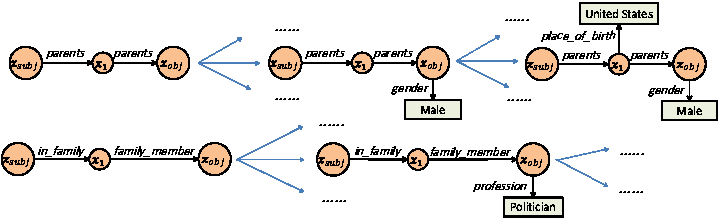
\includegraphics[width=1.0\columnwidth]{figure/schema/schema_gen-crop.eps}
    \bicaption{``has father'' 模式图挖掘示例。}{Candidate generation example of relation ``has father''.}
    \label{fig:schema-candgen}
\end{figure*}

在生成仅包含骨架的简单模式图之后,我们采用深度优先搜索的方式获取更多更加具体的模式图。
如\figref{fig:schema-candgen}所示,``has grandfater'' 关系可以生成多种不同的简单模式图,
在此基础上,我们逐步添加表示复杂语义的分支,让模式图更加具体。
这个步骤的挑战在于,即便骨架长度得到限制,模式图扩展的搜索空间仍然异常庞大。
%受Beam搜索\cite{ney1992improvements}的启发, 
为了提高效率,我们使用优先队列维护搜索过程中获取的高质量模式图,
并进行剪枝操作,压缩候选图的搜索空间。
具体步骤的伪代码流程如\algoref{alg:schema-dfs}所示。
$Q$为存放模式图的优先队列,初始化为空,最大容量为$B$,
搜索过程中始终维护具有最大支持率的前$B$个候选图(\lineref{line:pop})。
使用支持率作为剪枝依据的原因有二:
一方面如同骨架生成中的论述,支持率高的模式图更不容易偏离语义,
而支持率过低的候选图更有可能引入了不必要的限制,导致无法匹配大量已知三元组;
另一方面,随着候选图上添加的限制越多,支持率一定呈非严格单调递减趋势,
因此这种单调性特征可以直接用于剪枝。
函数$SchemaExpansion$以模式图$S$为输入,返回值为一个模式图集合,其中每个模式图均为
在$S$上加入一条新的限制所形成的更复杂的候选,
例如\figref{fig:schema-candgen}中的($x_{obj}$, $gender$, $Male$),
($x_{obj}$, $profession$, $Politician$)等。

%At each step of the search, We prune out $S$ if it has only a few supports, 
%or its support is smaller than any schemas stored in $Q$, when $Q$ is full.
%Otherwise, we add it into the priority queue, 
%then enumerate all the possible new schemas $S'$ (with one additional edge),
%and continue this searching step.
%Each additional edge on a variable node acts like a constraint on the variable.
%In practice, multiple constraints on the same variable seldom make sense. 
%Therefore, we require that at most one edge is added to any node 
%on the skeleton.

\begin{algorithm}
\caption{复杂模式图搜索}
\label{alg:schema-dfs}
\textbf{Input}: Schema $S$, priority queue $Q$, budget $B$, minimum support ratio $\gamma$ \\
\textbf{Output}: Priority queue $Q$ after expanding on $S$
\begin{algorithmic}[1]
\Procedure{Search}{$S, Q, B, \gamma$}
	\If {$sup(S) < \gamma$} 
		\State {\Return {$Q$}}	%\Comment{Skip $S$ due to low support}
	\EndIf
	\If {$Q.size < B$ or $sup(S) > sup(Q.top)$}
		\State {$Q.push(S)$}	%\Comment{Add $S$ into priority queue}
		\While {$Q.size > B$}
			\State {$Q.pop()$} \label{line:pop}%\Comment{Keep top-$B$ schemas}
		\EndWhile
		\State {$NewList \gets SchemaExpansion(S)$} \label{line:exp}
		\For {$S'$ in $ NewList $}
			\State {$Q \gets Search(S', Q, B, \gamma)$}
		\EndFor
	\EndIf
	\State \Return {$Q$}
\EndProcedure
\end{algorithmic}
\end{algorithm}


%At each step of the search, we enumerate all the possible new schemas
%(with one new edge) and insert the best among them to the priority queue if the
%queue is not full. If the queue is full, we compare the support of the 
%schema to be inserted with the worst schema on the queue. 
%If the current schema is better than the worst schema on the queue, 
%the worst schema is replaced and
%the search continued from the current best schema. 
%Otherwise, we prune the search space and backtrack.
%
%
%
%
%At each step of the search, we attempt to add an edge to any one node
%on the skeleton, which generates a more specific schema $S'$.
%A new edge is accepted if $sup(S') \ge \gamma$.
%%the support of the new schema is larger than $\gamma$. 
%This process continues recursively until
%no new schemas can be found.
%%3-6: basic limit on schema constraints
%%3. why need limitation
%%The searching space is a tree structure which grows exponentially,
%%making the exhaustive searching intractable on a huge knowlege base.
%%4. how to fix the search size
%Each additional edge on a variable node acts like a constraint on the variable.
%In practice, multiple constraints on the same variable seldom make sense. 
%Therefore, we require that at most one edge is added to any node 
%on the skeleton.
%%5. the intuition behind
%%As mentioned before, natural language relations are always short
%%phrases, which gives us the point that it's less likely to infer
%%a comfortable structure for a relation with multiple restriction 
%%imposed on a single element, and our restriction just follows 
%%this intuition.
%%6. the effect of limitation
%Consequently, the maximal depth of the searching tree is $\tau+1$.
%
%%7-11: budget base (why, budget+prune, criteria, how to prune, diversity)
%%7. why need budget
%Unfortunately, each node in a skeleton may be attached hundreds of
%different predicates in a large KB. The overall search space, though
%bounded by the constant depth, is still large.
%%8. introduce budget+pruning
%Inspired by beam search algorithm\cite{ney1992improvements}, 
%we introduce a fixed size 
%priority queue to store the set of candidate schemas for each relation.
%Our goal is to fill this queue (an operational budget) 
%with relatively higher quality
%schemas. We simply use the support of each schema on the input instances
%as the quality or priority of the schema. The idea is that a better schema
%should cover more instances. Also since as we attach more edges to the schema,
%the support monotonically decreases, we can use this 
%monotonicity property to prune the search
%space. At each step of the search, we enumerate all the possible new schemas
%(with one new edge) and insert the best among them to the priority queue if the
%queue is not full. If the queue is full, we compare the support of the 
%schema to be inserted with the worst schema on the queue. 
%If the current schema is better than the worst schema on the queue, 
%the worst schema is replaced and
%the search continued from the current best schema. 
%Otherwise, we prune the search space and backtrack.
%\KZ{The above description might be hard to understand without a simple
%pseudo-code.}

%while pruning strategies will be used to reduce 
%searching space so that poor candidates could be ignored.
%9. what's the criteria
%To this end, we use the number of instances covered by 
%a schema as the criteria to approximately measure its quality.
%%10. explanation of the criteria
%The reason is two-fold: we aim to keep those descriptive schemas in 
%the output candidates, since we output a bunch of schemas instead
%of only a few, we don't need a rather precise quality measurement,
%the idea that better schemas cover more positive instances is
%reasonable enough for our task; 
%and the size of coverages would never increase when the search goes
%deeper, which leads to a simple but effective pruning strategy.
%
%11-15. formal describe
%Now we explain the searching step in formal.
%% [A simple pseudo code is available]
%The beginning state of the searching is one skeleton, we enumerate
%all the constraints which are allowed to add on, each constraint 
%maps to a more specific schema.
%Then new schemas are ranked over their coverages by descending order,
%and we sequentially continue recursive searching on those schemas.
%When the searching state comes to a new schema $s_0$, we keep this 
%schema if there has enough room to keep candidates; 
%otherwise, we pick the schema $s_1$ which has the smallest 
%coverage among all kept schemas and compare their coverage.
%If $s_0$ has a larger coverage, then $s_1$ is discarded, we keep 
%$s_0$ and search deeper; otherwise, the current schema $s_0$ is 
%pruned, and we backtrace the searching process immediately.
%Finally, the output candidates are those schemas been kept when
%the searching is over.


为了使候选模式图之间具有多样性,
我们期望最终保留的$B$个候选图中能包含多种不同的骨架,
因为不同骨架的模式图通常代表更大的语义差别。
%TODO: 这是因为骨架的差别代表大的语义差别
%The diversity of output schemas plays an important rule in the 
%learning parts.
%If most candidates are the same and only differ from one or two 
%constraints, we are actually wasting budgets because it contains
%much redundant information.
因此在实际的搜索过程中,我们根据不同骨架的支持率,
将整个大小为$B$的优先队列按比例分为多块,
每个骨架上的深度搜索将使用各自独立的优先队列。
这样的做法可以提高并行工作效率,
同时保证候选集合不被某个高支持率的骨架主导。

%TODO:甩图,poster上面的
